% !TeX program = pdflatex
\documentclass[11pt,a4paper]{article}

\usepackage[margin=2.4cm]{geometry}
\usepackage{amsmath,amssymb,amsthm,mathtools}
\usepackage{graphicx}
\usepackage{booktabs}
\usepackage{hyperref}
\usepackage{cleveref}
\usepackage{microtype}
\usepackage{xcolor}

\hypersetup{colorlinks=true,linkcolor=blue!40!black,citecolor=blue!40!black,
            urlcolor=blue!40!black,pdftitle={Edge-disjoint triangulations of convex polygons}}

\newtheorem{theorem}{Theorem}[section]
\newtheorem{lemma}[theorem]{Lemma}
\newtheorem{proposition}[theorem]{Proposition}
\newtheorem{corollary}[theorem]{Corollary}
\theoremstyle{definition}
\newtheorem{definition}[theorem]{Definition}
\newtheorem{example}[theorem]{Example}
\theoremstyle{remark}
\newtheorem{remark}[theorem]{Remark}
\newtheorem{conjecture}[theorem]{Conjecture}

\newcommand{\P}{\ensuremath{P}}
\newcommand{\D}{\ensuremath{\mathcal{D}}}
\newcommand{\Z}{\ensuremath{\mathbb{Z}}}
\newcommand{\Li}{\mathrm{L}}
\newcommand{\Ri}{\mathrm{R}}

\title{\bfseries Edge-disjoint triangulations of convex polygons:\\
packing numbers, resolutions, and their classification}
\author{}
\date{}

\begin{document}
\maketitle

\begin{abstract}
How many triangulations of a convex $n$-gon can be drawn at the same time if no two of
them may share a diagonal?  We answer this exactly: the maximum is $\lfloor n/2\rfloor$,
for every $n\ge 4$.  For even $n=2m$ the extremal question becomes rigid and admits a
complete answer: every extremal family is a \emph{resolution}, that is, a partition of the
set of all $n(n-3)/2$ diagonals into $m$ \emph{snakes} (triangulations with no interior
triangle) whose $m$ pairs of ears partition the vertex set.  We then classify resolutions
by encoding a snake as a lattice path: a snake with prescribed endpoints corresponds
bijectively to a word in $\{\Li,\Ri\}^{n-4}$, the level (cyclic distance) of its
$i$-th strip diagonal is $\min(i+2,n-i-2)$ independently of that word, and $m$ snakes read
from one common word and based at the $m$ antipodal pairs $\{u,u+m\}$ partition all
diagonals if and only if the word is anti-palindromic, $w_i\ne w_{2m-3-i}$.  A resolution
whose $m$ snakes follow a common word is automatically antipodal, and conversely the number
of such resolutions of $P_{2m}$ is exactly $2^{m-2}$, in bijection with $\{0,1\}^{m-2}$.  We
conjecture that every resolution is of this form; this is verified exhaustively for
$m\le 7$ by exact-cover integer programming.  A generalisation to
$p$-angulations shows that the counting bound is sharp only for triangles.  Everything is
implemented, tested (188 tests) and verified computationally in the accompanying software.
\end{abstract}

\section{Introduction}

A triangulation of a convex polygon $P_n$ is a set of $n-3$ pairwise non-crossing
diagonals.  There are $C_{n-2}$ of them, where $C_j$ is the $j$-th Catalan number, and
their geometry is classical and well understood.  What is much less studied is what happens
when several triangulations have to coexist: how many of them can be drawn on the same
polygon without any two of them using a common diagonal?

This paper studies that question, and then goes further: instead of asking only for the
maximum size, we describe the structure of the extremal families and count them.

\paragraph{The question.}
For a family $\mathcal{T}$ of triangulations of $P_n$ we call it a \emph{$k$-packing} if
$|\mathcal{T}|=k$ and no two members share a diagonal, and we write
\[
  M(n)\;=\;\max\{k : \text{$P_n$ admits a $k$-packing}\}.
\]
The answer is
\[
  \boxed{\,M(n)=\lfloor n/2\rfloor \quad\text{for all } n\ge4\,} \tag{0}
\]
The upper bound is a one-line consequence of the two-ears property and a counting
argument on the short diagonals (\cref{thm:packing-number}); sharpness is explicit.

\paragraph{Why the even case is the interesting one.}
If $n=2m$ then a family of $m$ pairwise edge-disjoint triangulations uses
$m(2m-3)=|\D_{2m}|$ diagonals, i.e.\ \emph{every} diagonal; and since each triangulation
must use at least two of the $2m$ short diagonals $(v-1,v+1)$, each of them uses exactly
two, hence has exactly two ears and no interior triangle.  So for even $n$ an extremal
family is forced to be a partition of all diagonals into snakes (\cref{prop:structure}).
This is a strong rigidity statement, and it is what makes a classification possible.

\paragraph{Contributions.}
\begin{itemize}
\item[\textbf{T1.}] $\ M(n)=\lfloor n/2\rfloor$ for all $n\ge 4$ (\cref{thm:packing-number}),
with explicit optimal families for even and odd $n$.
\item[\textbf{T2.}] For $n=2m$, every $m$-packing is a \emph{resolution}: a partition of
$\D_{2m}$ into $m$ snakes whose $m$ ear pairs partition the vertex set
(\cref{prop:structure}).
\item[\textbf{L3.}] A bijection between snakes of $P_n$ with prescribed endpoints and
words $w\in\{\Li,\Ri\}^{n-4}$, together with two structural consequences: the endpoints
satisfy $v=u+\#\Ri(w)+2$, and the level of the $i$-th strip diagonal is
$\min(i+2,n-i-2)$, \emph{independently of the word} (\cref{lem:strip}).  In particular
$P_n$ has exactly $n\,2^{n-5}$ snakes.
\item[\textbf{T4.}] Let $n=2m\ge 6$ and let $w\in\{\Li,\Ri\}^{2m-4}$ have exactly $m-2$
letters $\Ri$.  The $m$ snakes based at the antipodal pairs $\{u,u+m\}$ and read from $u$
partition all diagonals of $P_{2m}$ if and only if $w_i\ne w_{2m-3-i}$ for all
$1\le i\le m-2$ (\cref{thm:classification}).  Every resolution whose $m$ snakes follow a
common word is of this form and is automatically antipodal (\cref{cor:count}(i)), so the
number of such resolutions is exactly $2^{m-2}$, in bijection with $\{0,1\}^{m-2}$
(\cref{cor:count}(ii)).
\item[\textbf{T5.}] Exact values of the number of $k$-packings for $n\le 10$, e.g.\ 
$2\,436$ pairs and $2\,472$ triples of edge-disjoint triangulations of $P_8$ ($=4$
quadruples).
\item[\textbf{T6.}] A $p$-angulation generalisation: a $p$-angulation of $P_n$ exists iff
$(p-2)\mid(n-2)$, and the naive counting bound on edge-disjoint $p$-angulations is
\emph{not} attained for $p\ge4$ (e.g.\ $4$ instead of $10$ for $P_8$,
\emph{Proposition~\ref{prop:p-angulations}}).
\item[\textbf{C1.}] \emph{Conjecture.} Every resolution of $P_{2m}$ follows a common word
(and is therefore antipodal).  Verified exhaustively for $m\le 7$; see
\cref{sec:experiments}.
\end{itemize}

\paragraph{What is proved where.}
\Cref{thm:classification} is the paper's main result and is proved in \cref{sec:proofs} by a
covering argument on the layers of diagonals of equal level.  Everything else follows from
it, except Conjecture~C1, which we do not prove; \cref{sec:limits} states precisely what
that means for the counting result.

\section{Related work and novelty}

We are not aware of prior work on $M(n)$.  A literature search (arXiv API, Semantic
Scholar, MathSciNet-style keyword searches, GitHub) for the phrases \emph{edge-disjoint
triangulations}, \emph{edge-disjoint triangulations of a convex polygon},
\emph{simultaneous triangulations}, \emph{partition of the diagonals into triangulations}
and \emph{perfect $k$-dissections} did not turn up a paper, theorem or OEIS entry about
this packing number or about such partitions.  We therefore state the claim carefully:
\emph{we did not find a prior result establishing (0), the structure theorem T2, or the
classification T4.}  We do not claim priority.

The classical ingredients we build on are the following.
\begin{itemize}
\item The number of triangulations of a convex $n$-gon is the Catalan number $C_{n-2}$
(OEIS \href{https://oeis.org/A000108}{A000108}); we only use the count, never the formula.
\item Every triangulation of a convex polygon has at least two \emph{ears}, i.e.\ triangles
with two sides of the polygon.  We prove the version we need in \cref{lem:ears} (via the
dual tree) rather than citing the ``two ears theorem'', so the paper is self-contained.
\item \emph{Snakes} --- triangulations of a convex polygon with no interior triangle, dual
graph a path --- are a standard object (sometimes called \emph{path} or \emph{serpentine}
triangulations).  We use the fact that there are $n\,2^{n-5}$ of them, but we prove it in
\cref{lem:snakes} from our own encoding, because the standard reference for it did not
list the object in a form we could cite precisely.
\item A dissection of a convex $n$-gon into $p$-gons exists iff $(p-2)\mid(n-2)$; this
follows immediately from Euler's formula and we prove it in
\cref{prop:p-angulations}.
\item Integer programming is used only as an exact computational device: the packing
problem and the completeness check of Conjecture~C1 are set-partitioning problems solved by
HiGHS \cite{huangfu2018} through \textsc{scipy} \cite{virtanen2020}.
\end{itemize}

\section{Preliminaries}

\begin{definition}[\label{def:poly}]
($P_n$, vertices, levels, sides, diagonals)
Let $P_n$ be a convex polygon with vertices labelled $0,1,\dots,n-1$ in cyclic order,
arithmetic on labels being modulo $n$.  Two chords cross if their endpoints interleave.
The \emph{level} of a diagonal $d=(i,j)$ ($i<j$) is
$\operatorname{lev}(d)=\min(j-i,\,n-(j-i))$, and its $i$-th and $j$-th endpoints are its
\emph{near} and \emph{far} endpoint resp.\ for $i<j$.  The $n$ diagonals of level $2$,
\[
  s_v=(v-1,v+1)\qquad (v\in\Z_n),
\]
are the \emph{short diagonals}; $s_v$ \emph{cuts off the vertex $v$}, which we call its ear
vertex.
\end{definition}

\begin{definition}
A \emph{triangulation} of $P_n$ is a maximal set of pairwise non-crossing diagonals; it
consists of $n-3$ diagonals and $n-2$ triangles.  The \emph{dual graph} of a triangulation
has one vertex per triangle and one edge per diagonal of the triangulation, joining the two
triangles it separates; it is connected (one can walk from any triangle to any other across
diagonals) and has $n-3$ edges on $n-2$ vertices, hence it is a tree.
\end{definition}

\begin{definition}
An \emph{ear} of a triangulation is a triangle with two sides of $P_n$.  A vertex $v$ is
an \emph{ear vertex} if the triangle $(v-1,v,v+1)$ is part of the triangulation; this
happens iff $s_v$ is a diagonal of the triangulation.  A triangulation with no triangle all
three of whose edges are diagonals is called a \emph{snake} (its dual graph is a path).
\end{definition}

\begin{lemma}[\label{lem:ears}]
Every triangulation of $P_n$ has at least two ears, and it is a snake if and only if it has
exactly two ear vertices.
\end{lemma}

\begin{proof}
The dual graph is a tree with $n-2\ge2$ vertices and hence at least two leaves.  A leaf of
the dual graph corresponds to a triangle adjacent to only one diagonal, hence to a triangle
with two sides of $P_n$, i.e.\ an ear.  Each ear vertex $v$ contributes exactly one ear and
$s_v\in T$ iff $v$ is an ear vertex, so the number of ears equals the number of short
diagonals in $T$.  Finally, a triangulation has no interior triangle iff its dual tree has
no vertex of degree $3$, i.e.\ iff the tree is a path, i.e.\ iff it has exactly two leaves.
\end{proof}

\begin{definition}
A family of triangulations is \emph{edge-disjoint} if no two members share a diagonal.
A \emph{$k$-packing of $P_n$} is an edge-disjoint family of $k$ triangulations.
A \emph{resolution of $P_{2m}$} is a family of $m$ snakes that partitions $\D_{2m}$, the set
of all diagonals of $P_{2m}$.  A snake is \emph{antipodal} if its two ear vertices are at
cyclic distance $m$.  A resolution is \emph{antipodal} if all of its snakes are.
\end{definition}

\section{The packing number}

\begin{theorem}[\label{thm:packing-number}]
For every $n\ge4$ the maximum size of an edge-disjoint family of triangulations of $P_n$
is
\[
  M(n)=\Big\lfloor\frac n2\Big\rfloor .
\]
\end{theorem}

\begin{proof}
\emph{Upper bound.}  Assume $n\ge5$ (for $n=4$ the bound $k\le2$ is trivial, $P_4$ having
exactly two triangulations).  Let $\mathcal{T}$ be an edge-disjoint family of $k$
triangulations of $P_n$.  By \cref{lem:ears} each $T\in\mathcal{T}$ contains at least two
short diagonals.  Distinct members of $\mathcal{T}$ use disjoint sets of short diagonals, and
there are $n$ of them, so $2k\le n$, i.e.\ $k\le\lfloor n/2\rfloor$.

\emph{Sharpness, $n=2m$.}  Let $w_0=\Ri^{m-2}\Li^{m-2}$ and, for $u\in\Z_m$, let $T_u$ be
the snake of $P_{2m}$ whose endpoints are $u$ and $u+m$ and whose word is $w_0$ (it exists
and is unique by \cref{lem:strip}(iii)).  The word $w_0$ satisfies
$w_{0,i}\ne w_{0,\,2m-3-i}$ for $1\le i\le m-2$, so \cref{thm:classification} gives that
$\{T_u\}_{u\in\Z_m}$ is a resolution of $P_{2m}$, in particular an $m$-packing.

\emph{Sharpness, $n=2m-1\ge5$.}  Take the same resolution of $P_{2m}$ and delete the vertex
$2m-1$, obtaining $P_{2m-1}$ (the labelling of the remaining vertices is unchanged).  For a
triangulation $T$ of $P_{2m}$ write $d_T(x)$ for the number of diagonals of $T$ meeting
$x$.  By \cref{lem:delete} the diagonals of $T$ that survive the deletion form a
triangulation of $P_{2m-1}$ as soon as $d_T(x)\le1$.  The snake $T_u$ of $w_0$ is the union
of the fan at $u-1$ (the diagonals $(u-1,u+1),\dots,(u-1,u+m-1)$) and the fan at
$u-1+m$ (the diagonals $(u-1+m,u+m+1),\dots,(u-1+m,u+2m-2)$), so
\[
  d_{T_u}(2m-1)=\begin{cases}m-1,&u=0,\\ 1,&1\le u\le m-2,\\ 0,&u=m-1,\end{cases}
\]
the first line because $u-1=2m-1$ is the hub of the first fan, and the second because
$u+m+1\le 2m-1\le u+2m-2$ holds exactly when $1\le u\le m-2$.  In particular
$d_{T_u}(2m-1)\le1$ for every $u\ne0$, so $T_1,\dots,T_{m-1}$ each become a triangulation of
$P_{2m-1}$, and they remain pairwise edge-disjoint because they were.  This gives an
$(m-1)$-packing.  For $n=4$ the two triangulations of the square are edge-disjoint.
\end{proof}

\begin{lemma}[\label{lem:delete}]
Let $T$ be a triangulation of $P_n$ and let $x$ be a vertex with $d_T(x)\le1$.  Delete $x$
together with all diagonals meeting $x$ and with $s_x$ (which becomes a side of
$P_{n-1}$).  The remaining set is a triangulation of $P_{n-1}$.
\end{lemma}

\begin{proof}
If $d_T(x)=0$ then $x$ is an ear vertex and the only triangle at $x$ is $(x-1,x,x+1)$; if
$d_T(x)=1$ the unique diagonal at $x$ is $s_x$ and the triangles at $x$ are
$(x-1,x,x+1)$ and $(x-1,x+1,y)$ for some $y$.  In both cases the triangles not containing
$x$ are unchanged and none of them is lost, and their number drops from $n-2$ to $n-3$,
which is the number of triangles of $P_{n-1}$; their diagonals are exactly the survivors.
\end{proof}

\begin{example}
The canonical resolution of $P_8$ (word $w_0=\Ri\Ri\Li\Li$) consists of the four snakes
\[
\begin{aligned}
  T_0&=\{(1,7),(2,7),(3,5),(3,6),(3,7)\},\\
  T_1&=\{(0,2),(0,3),(0,4),(4,6),(4,7)\},\\
  T_2&=\{(0,5),(1,3),(1,4),(1,5),(5,7)\},\\
  T_3&=\{(0,6),(1,6),(2,4),(2,5),(2,6)\},
\end{aligned}
\]
with ear pairs $\{0,4\},\{1,5\},\{2,6\},\{3,7\}$; the eight diagonals they use are distinct
and together exhaust the $20$ diagonals of $P_8$.
Figure~\ref{fig:canonical} draws the same structure for $P_{10}$.
\end{example}

\section{Snakes as lattice paths}

\begin{lemma}[\label{lem:strip}]
Let $n\ge5$ and let $u$ be an ear vertex of a snake $T$ of $P_n$, the other ear vertex
being $v$.  Then:
\begin{enumerate}[(i)] $v=u+\#\Ri(w)+2$ for a word $w\in\{\Li,\Ri\}^{n-4}$ with
$\#\Li(w)=n-4-\#\Ri(w)$; in particular $v$ is determined by $\#\Ri(w)$;
\item the $i$-th diagonal met by the strip of $T$ read from $u$ has level
$\min(i+2,n-i-2)$, $i=0,\dots,n-4$;
\item snakes with endpoints $u,v$ are in bijection with words in
$\{\Li,\Ri\}^{n-4}$ having $\#\Ri=v-u-2$ letters $\Ri$; in particular $P_n$ has exactly
$n\,2^{n-5}$ snakes.
\end{enumerate}
\end{lemma}

\begin{proof}
\emph{The encoding.}  The triangles of $T$ form a path in the dual graph, so $T$ has a
\emph{strip}: an ordering $t_0,t_1,\dots,t_{n-3}$ of its triangles in which consecutive
triangles share a diagonal.  Write $b_i$ for the boundary edge of $t_i$.  Because no
triangle of $T$ is interior, each $t_i$ has at least one boundary edge, and exactly the two
end triangles $t_0,t_1$---the ears---have two; consequently each $b_i$ is a distinct
boundary edge and all $n$ of them are used.  Moreover, at every internal triangle, the
boundary edge is the one immediately following $b_{i-1}$ or the one immediately preceding
it in cyclic order: the consumed boundary edges always form an arc containing $b_0,b_1$.
Encode the choice at step $i$ ($2\le i\le n-3$) by $\Li$ if the arc grows counterclockwise
and by $\Ri$ if it grows clockwise, obtaining $w\in\{\Li,\Ri\}^{n-4}$.  Let $L_i,R_i$ be the
numbers of $\Li$'s and $\Ri$'s among the first $i$ letters, so $L_i+R_i=i$.  The consumed
arc is $\{$ vertices $u-1-L_i,\dots,u+1+R_i\}$ at that moment, and its endpoints are joined
by the diagonal
\[ F_i=\{\,u-1-L_i,\;u+1+R_i\,\},\qquad i=0,1,\dots,n-4. \tag{1} \]
$F_0=s_u$ and $F_{n-4}=s_v$.  This construction is reversible, so it is a bijection between
snakes with ear vertex $u$ and words of length $n-4$.

\emph{(i)} Put $a=\#\Li(w)$ and $b=\#\Ri(w)$, so $a+b=n-4$.  Then
$F_{n-4}=\{u-1-a,\;u+1+b\}$, and since
\[
  \{u-1-a,u+1+b\}=\{v-1,v+1\}
\]
with $a+b+2\equiv0 \pmod n$ (because $a+b=n-4$ and $n\mid 2(a+b+4)$), the matching is the
crossed one: $v-1=u+1+b$ and $v+1=u-1-a$, whence $v=u+b+2=u+\#\Ri(w)+2$.

\emph{(ii)} The two endpoints of $F_i$ differ by $(u+1+R_i)-(u-1-L_i)=2+L_i+R_i=i+2$, so
$\operatorname{lev}(F_i)=\min(i+2,n-i-2)$, which does not involve the word.

\emph{(iii)} Immediate from the bijection: for fixed $u$ and $b=v-u-2$ there are
$\binom{n-4}{b}$ snakes.  Counting pairs $(T,\text{chosen ear vertex})$ we get
$\sum_{u\in\Z_n}\sum_{b=0}^{n-4}\binom{n-4}{b}=n\,2^{n-4}$, and since a snake has exactly two
ear vertices for $n\ge5$, the number of snakes is $n\,2^{n-5}$.
\end{proof}

\begin{corollary}
In any edge-disjoint family of triangulations of $P_n$ in which every member is a snake,
each snake uses exactly two of the $n$ short diagonals, and the ear vertices of the
snakes are pairwise distinct.
\end{corollary}

\begin{proof}
Each snake uses at least two short diagonals (\cref{lem:ears}), and distinct members use
disjoint sets of the $n$ available short diagonals.
\end{proof}

\section{Main results}

\subsection{Classification of the common-word resolutions}

\begin{theorem}[\label{thm:classification}]
Let $n=2m\ge6$ and let $w\in\{\Li,\Ri\}^{2m-4}$ have exactly $m-2$ letters $\Ri$.  For
$u\in\Z_m$ let $T_u$ be the snake of $P_{2m}$ with endpoints $u$ and $u+m$ and with word
$w$ (which exists and is unique by \cref{lem:strip}).  Then
\[
  \{T_u : u\in\Z_m\}\ \text{ is a resolution of } P_{2m}
  \quad\Longleftrightarrow\quad
  w_i\ne w_{2m-3-i}\ \text{ for all } 1\le i\le m-2 . \tag{2}
\]
\end{theorem}

\begin{corollary}[\label{cor:count}]
\begin{enumerate}[(i)] Every resolution of $P_{2m}$ whose $m$ snakes follow a \emph{common
word} (each read from one of its ear vertices) is antipodal, and is of the form of
\cref{thm:classification}.
\item[$(ii)$] For $m\ge2$ there are exactly $2^{m-2}$ such resolutions, and
$w\mapsto\{T_u\}_{u\in\Z_m}$ is a bijection from the set of anti-palindromic words
$w\in\{\Li,\Ri\}^{2m-4}$ onto them.  Equivalently they are in bijection with
$\{0,1\}^{m-2}$, the free first half of the word.
\end{enumerate}
\end{corollary}

\begin{proof}
(i) Let $\mathcal{T}$ be a resolution all of whose snakes follow the common word $w$, and put
$b=\#\Ri(w)$ and $k=b+2$.  By \cref{lem:strip}(i) every ear pair of $\mathcal{T}$ then has
cyclic length $k$, and by \cref{prop:structure}(iii) these $m$ pairs partition $\Z_{2m}$.
Write $\ell_i$ for the number of $\Li$'s among the first $i$ letters of $w$ and
$\widehat\rho_i$ for the number of $\Ri$'s among the last $i$; both are independent of the
snake because $w$ is common.  For $i\in\{0,\dots,m-3\}$ with $j=i+2\le m-1$, the computation
of \cref{sec:proofs} (with $u$ ranging over the $m$ arc-start vertices rather than over
$\Z_m$) shows that the $2m$ starts of the diagonals at level $j$ are
\[
  A=\{u-1-\ell_i\},\qquad B=\{u+k-1-\widehat\rho_i\}=A+\big(k-\widehat\rho_i+\ell_i\big).
\]
Since $\mathcal{T}$ is a resolution, $A\sqcup B=\Z_{2m}$.  Now $A$ is a block of $m$
consecutive residues, and the complement of such a block in $\Z_{2m}$ is its translate by
$m$; hence
$k-\widehat\rho_i+\ell_i\equiv m\pmod{2m}$.  Comparing this with the conclusion of
\cref{sec:proofs} in the ($\Rightarrow$) direction, namely
$L_i=\widehat\rho_i$ for every $i\le m-3$ (which uses only the level conditions and the
commonality of the word), we get $k\equiv m\pmod{2m}$.  Since $2\le k\le n-1$ and
$1\le m\le n/2$, this forces $k=m$: every ear pair is antipodal, and \cref{lem:strip}(i)
then gives $\#\Ri(w)=m-2$, so $\mathcal{T}$ is precisely the family of
\cref{thm:classification} for $w$.
(For $m\le3$ there is no admissible level $i$; $m=2$ gives $\mathcal{T}$ the two
triangulations of $P_4$ and $m=3$ follows from \cref{lem:strip}(i) and
\cref{prop:structure}(iii): the three pairs of length $k$ partitioning six vertices force
$k=3$.)

(ii) By \cref{thm:classification} the common-word resolutions are exactly those produced by
anti-palindromic words.  Condition (2) forces one letter of each pair
$(i,\,2m-3-i)$, $1\le i\le m-2$, so the first $m-2$ letters determine the rest; conversely
any choice of the first $m-2$ letters extends to exactly one word satisfying (2), and that
word automatically has $m-2$ letters $\Ri$ and $m-2$ letters $\Li$.  Distinct words give
distinct resolutions because the word is recovered from the resolution
(\cref{cor:recover}).  Hence the count is $2^{m-2}$.
\end{proof}

\begin{corollary}[\label{cor:recover}]
The word of a resolution is determined by the resolution: if $R=\{T_u\}$ is an
common-word resolution then the words of all $T_u$ (read from $u$) agree.
\end{corollary}

\begin{proof}
Immediate from the bijection in \cref{cor:count}, or directly: given $T_u$ and its ear
vertex $u$, the word is recovered by \cref{lem:strip}'s construction, which is invertible.
\end{proof}

\subsection{Structure of extremal families}

\begin{proposition}[\label{prop:structure}]
Let $n=2m\ge6$.  If $\mathcal{T}$ is an $m$-packing of $P_{2m}$ then:
\begin{enumerate}[(i)] $\bigcup_{T\in\mathcal{T}}T=\D_{2m}$, i.e.\ $\mathcal{T}$ is a
resolution;
\item every $T\in\mathcal{T}$ is a snake with exactly two ears;
\item the $m$ pairs of ear vertices of $\mathcal{T}$ partition $\Z_{2m}$.
\end{enumerate}
\end{proposition}

\begin{proof}
(i) $|\D_{2m}|=m(2m-3)$ and each member uses $2m-3$ diagonals, so $m$ edge-disjoint members
use all of them.  (ii) Each member uses at least two short diagonals, the $m$ members use at
least $2m$, and there are exactly $2m$ short diagonals; hence each uses exactly two, so by
\cref{lem:ears} it has exactly two ears and is a snake.  (iii) Each of the $2m$ short
diagonals is used exactly once, and $s_v$ is used by the snake having $v$ as an ear
vertex, so the $m$ ear pairs are disjoint and cover $\Z_{2m}$.
\end{proof}

\begin{remark}
Proposition~\ref{prop:structure} is what makes \cref{thm:classification} the natural
classification problem: for even $n$ there is no choice about \emph{what} an extremal
family is, only about \emph{which} one it is.
\end{remark}

\section{Proofs of the main theorems}\label{sec:proofs}

Throughout, $n=2m$ with $m\ge3$, $w\in\{\Li,\Ri\}^{2m-4}$ has exactly $m-2$ letters
$\Ri$, and $T_u$ is as in \cref{thm:classification}.  For $0\le i\le n-4$ we abbreviate
$L_i=L_i(w)$ and $R_i=R_i(w)$, and we use the following notation.

\medskip
\noindent\textit{Levels.}  For $2\le j\le m-1$ there are exactly $2m$ diagonals of level
$j$, namely $\{x,x+j\}$ for $x\in\Z_{2m}$; for $j=m$ there are $m$ of them, the
\emph{diameters} $\{x,x+m\}$ for $x\in\Z_m$.  By \cref{lem:strip}(ii) the strip diagonal
$F_i$ of $T_u$ has level $\min(i+2,n-i-2)$, so each snake contains exactly two diagonals of
each level $j<m$ (at strip positions $i=j-2$ and $i=n-2-j$) and exactly one diameter (at
strip position $i=m-2$).

\medskip
\noindent\textit{Condition \textup{(CP)}.}  Throughout, positions of a word are numbered
$1,2,\dots,2m-4$.  Say that $w$ satisfies the \emph{covering property} if
\[
  w_i \ne w_{n-3-i}\quad\text{for } i=1,\dots,m-2, \tag{CP}
\]
i.e.\ if the letters in positions $i$ and $n-3-i$ differ; this is condition (2), which
reads $w_i\ne w_{2m-3-i}$ when written in the theorem statement.

\medskip
\noindent\textit{Key observation.}  Assume (CP) and fix $i$ with $0\le i\le m-3$; put
$c=L_i$ and, for $t\in\{1,\dots,m-2\}$, let $\rho_t$ be the indicator that the letter in
position $n-3-t$ is $\Ri$.  Then
\[
  \rho_t=1-\ell_t,\qquad
  L_i=\sum_{t\le i}\ell_t,\qquad
  \widehat{\rho}_i:=\#\{\Ri\text{ among the last } i \text{ letters}\}
     =\sum_{t\le i}\rho_t=i-L_i , \tag{3}
\]
because the last $i$ positions are exactly $\{n-3-t:1\le t\le i\}$ (as $i\le m-3$ ensures
$n-3-i\ge m$), i.e.\ they are precisely the partners of the first $i$ positions under
(CP).  In particular $\widehat\rho_i=L_i$, and more generally
$L_{i'}-L_i=\widehat\rho_{i'}-\widehat\rho_i$ for $i\le i'\le m-3$: the number of $\Li$'s
among the first $i'$ letters equals the number of $\Li$'s among the last $i'$ letters.

\begin{proof}[\textit{Proof of \cref{thm:classification}}]
By \cref{lem:strip}(ii) the $2m$ strip diagonals of the family at the two positions $i$ and
$n-2-i$ have level $j=i+2$.  Write $\alpha_u$ for the \emph{start} of the position-$i$
diagonal of $T_u$, i.e.\ the unique residue $x$ with $F_i=\{x,x+j\}$; by (1) and $i+2=j<m$
\[
  \alpha_u=u-1-L_i . \tag{4}
\]
Similarly, the position-$(n-2-i)$ diagonal of $T_u$ is $\{y_u,y_u+j\}$ with, using (1) and
the fact that its endpoints differ by $n-j$,
\[
  y_u=u+1+R_{n-2-i}=u+1+\big(\#\Ri-\widehat\rho_i\big)=u+m-1-\widehat\rho_i . \tag{5}
\]
Hence
\[
  y_u-\alpha_u=m+L_i-\widehat\rho_i . \tag{6}
\]

\emph{($\Leftarrow$.)}  Assume (CP).  By (3), $\widehat\rho_i=L_i$ for every
$i\le m-3$, so (6) gives $y_u=\alpha_u+m$.  The sets
\[
  A=\{\alpha_u:u\in\Z_m\}=\{u-1-c:0\le u<m\},\qquad
  B=\{y_u:u\in\Z_m\}=\{u+m-1-c:0\le u<m\}
\]
are therefore two disjoint intervals of $\Z_{2m}$ with $A\sqcup B=\Z_{2m}$: the $2m$ diagonals
at level $j$ are exactly the $2m$ diagonals of that level, each once.  The remaining level,
$j=m$, is automatic: the $m$ strip diagonals at position $m-2$ are $m$ distinct diameters
(the family is edge-disjoint) and there are exactly $m$ diameters.  So every diagonal of
$P_{2m}$ is used exactly once and $\{T_u\}$ is a resolution.

\emph{($\Rightarrow$).)}  Suppose $\{T_u\}$ is a resolution.  Then for each
$i\in\{0,\dots,m-3\}$ the $2m$ starts of the diagonals at level $i+2$ are exactly
$\Z_{2m}$, so with $A,B$ as in (4), (5),
\[
  A\sqcup B=\Z_{2m},\qquad A=\{u-1-L_i\},\quad B=\{u+m-1-\widehat\rho_i\}=A+\delta,
\]
where $\delta=m+L_i-\widehat\rho_i$ by (6).  Now $A$ is an interval of $m$ consecutive
residues, and a translate of an interval of $m$ consecutive residues is its complement in
$\Z_{2m}$ only if the translation is $\equiv m\pmod{2m}$.  Hence
$\delta\equiv m\pmod{2m}$, i.e.\ $L_i\equiv\widehat\rho_i\pmod{2m}$, and since
$0\le L_i,\widehat\rho_i\le i\le m-3$ we get
\[
  L_i=\widehat\rho_i\qquad(0\le i\le m-3). \tag{7}
\]
Taking consecutive differences in (7), for $1\le i\le m-3$ we obtain
$\ell_i=\rho_i$, i.e.\ the letters in positions $i$ and $n-3-i$ of $w$ differ.  Finally,
$w$ has $m-2$ letters $\Li$, and the $m-3$ pairs just found already account for $m-3$ of
them, so the two remaining positions, $m-2$ and $m-1$ (1-based), contain exactly one
letter $\Li$; hence their letters differ as well.  This is (CP), i.e.\ (2).
\end{proof}

\begin{remark}
The two directions of \cref{thm:classification} use quite different amounts of
information: the ($\Leftarrow$) direction only needs, at each level, that the $2m$ starts
split into two complementary blocks of consecutive residues, which (CP) forces; the
($\Rightarrow$) direction needs only the trivial fact that a complement of an interval of $m$
consecutive residues is a translate by $m$.  No global or inductive argument is used, which
is why the criterion is a single anti-palindromicity condition.
\end{remark}

\section{Counterexamples, and the limits of what we prove}\label{sec:limits}

\subsection{The counting bound for $p$-angulations is not sharp}

The proof of the upper bound in \cref{thm:packing-number} counts short diagonals.  For
$p$-angulations there is no analogue, and pure diagonal counting fails.

\begin{proposition}[\label{prop:p-angulations}]
Let $p\ge3$.  (i) A $p$-angulation of $P_n$ exists iff $(p-2)\mid(n-2)$, and then it has
$(n-2)/(p-2)$ cells and $(n-p)/(p-2)$ diagonals.  (ii) Any family of pairwise
edge-disjoint $p$-angulations of $P_n$ has size at most
$\Big\lfloor \dfrac{n(n-3)/2}{(n-p)/(p-2)}\Big\rfloor$, and this bound is attained for
$p=3$ (\cref{thm:packing-number}) but not for $p\ge4$: for $p=4$ the optimum is
$3,4,5$ for $n=6,8,10$ respectively, against the bounds $9,10,11$.
\end{proposition}

\begin{proof}
(i) If $D$ is a set of $p$-angulation diagonals and $F$ the number of cells, then counting
side incidences gives $pF=2D+n$ and Euler's formula gives $F=D+1$; hence $D(p-2)=n-p$,
$F(p-2)=n-2$, so $(p-2)\mid(n-2)$ is necessary, and the constructions in
\cref{lem:p-angulation-exists} show it is sufficient.  (ii) The upper bound is diagonal
counting; the values are computed exactly by integer programming
(\cref{sec:experiments}) and, for $n=6$, also by hand: the only quadrangulations of a
hexagon use the three long diagonals $(0,3),(1,4),(2,5)$, one each, so at most three are
edge-disjoint, while diagonal counting would allow $\lfloor 9/2\rfloor=4$.
\end{proof}

\begin{lemma}[\label{lem:p-angulation-exists}]
If $(p-2)\mid(n-2)$ then $P_n$ has a $p$-angulation.
\end{lemma}

\begin{proof}
Write $n-2=(p-2)q$.  Induct on $q$.  For $q=1$, $n=p$ and the empty set of diagonals works.
For $q>1$, take the fan of $P_n$ at vertex $0$: its cells $(0,i,i+1)$, $1\le i\le n-2$, have
sides $i+2$; cutting this fan with $q-1$ further diagonals is equivalent to dissecting
$P_{n-1}$ (the polygon $1,\dots,n-1$) into cells of size $p$, which is possible by
induction because $(p-2)\mid(n-3)$.
\end{proof}

\begin{remark}
Part (ii) of \cref{prop:p-angulations} is a genuine obstruction to a naive generalisation:
for triangles the short-diagonal argument is exactly what closes the gap between counting and
truth, and for $p\ge4$ no analogous certificate is available.  We do not determine the
optimum for $p\ge4$ in general.
\end{remark}

\subsection{Conjecture C1: do all resolutions follow a common word?}

\begin{conjecture}
Every resolution of $P_{2m}$ follows a common word: there is a word
$w\in\{\Li,\Ri\}^{2m-4}$ such that all $m$ of its snakes, read from their clockwise-first
ear vertices, follow $w$.  In particular (by \cref{cor:count}(i)) every resolution is
antipodal.
\end{conjecture}

If C1 holds, then by \cref{cor:count} the number of resolutions of $P_{2m}$ is exactly
$2^{m-2}$ and the classification in \cref{thm:classification} is complete.  We can prove
Conjecture C1 for $m=3$ ($P_6$: by \cref{prop:structure}(iii) the three ear pairs partition
the six vertices, and a pair at cyclic distance $2$ forces the snake to be a fan, whose
$n-3$ diagonals all meet one vertex and which therefore cannot coexist with another
snake), and we verify it exhaustively for $m\le7$; see \cref{sec:experiments}.  We do
\emph{not} prove it for general $m$.

What we can say about where a proof would have to go.  Suppose a resolution is given with
snakes $S_u$ having ear pairs $\{a_u,b_u\}$, the pairs partitioning $\Z_{2m}$.  For each
level $i\in\{0,\dots,m-3\}$ the $2m$ strip starts must cover $\Z_{2m}$; the starts of
$S_u$ are $a_u-1-\ell^{(u)}_i$ and $b_u-1-\hat\rho^{(u)}_i$ (by the computation in
\cref{sec:proofs} with $a_u$ and $b_u$ in place of $u$ and $u+m$).  If $S_u$ were read from
$b_u$ instead, its word would have the same length and the same number of $\Ri$'s.  The
difficulty is that the $\ell^{(u)}_i$ and $\hat\rho^{(u)}_i$ now depend on $u$, so the
``interval and its translate'' argument of \cref{sec:proofs} no longer applies and a
consistency argument across all levels is needed.  Our partial analysis shows that the
level-$1$ condition forces all snakes to agree on their first and last move, and the
level-$2$ condition forces agreement on the second and second-to-last move; the induction
that would propagate this to all $2m-4$ positions breaks when the common prefix and the
common suffix contribute letters of different parity to $\sum_u(\ell_i+\hat\rho_i)$, which
is precisely where our argument stops.  We record this as the honest gap.

\section{Computational experiments}\label{sec:experiments}

All experiments are deterministic (no random seeds are needed) and are regenerated by
\texttt{python experiments/run\_all.py}.  Exact numbers below are copied from the files in
\texttt{results/}.

\paragraph{Enumeration cross-validation.}  The enumerator for dissections, triangulations
and $p$-angulations is implemented recursively (decomposition at the side $(0,n-1)$) and is
cross-checked against two independent methods: the Catalan numbers for triangulations, and
brute force over subsets of diagonals combined with an independent face-tracing routine for
$p$-angulations.  For $p=4$ this gives the sequence $1,3,12,55,273$ quadrangulations of
$P_4,P_6,\dots,P_{12}$.

\paragraph{Packing numbers and $k$-packing counts.}
\Cref{tab:small} lists, for $4\le n\le16$: the number of triangulations, the number of
snakes, $M(n)$ (which equals $\lfloor n/2\rfloor$ in every case, and agrees with the
optimum of the packing ILP for $n\le12$), the number of resolutions when $n$ is even, and
the exact number of $k$-packings for $n\le10$.

\begin{table}[h]
\centering\small
\begin{tabular}{rrrrrrrrr}
\toprule
$n$ & \#triangulations & \#snakes & $M(n)$ & \#resolutions & $k{=}2$ & $k{=}3$ & $k{=}4$ & $k{=}5$\\
\midrule
4  & 2       & 2    & 2 & 1  & 1     & --     & --     & --\\
5  & 5       & 5    & 2 & --  & 5     & --     & --     & --\\
6  & 14      & 12   & 3 & 2  & 34    & 2      & --     & --\\
7  & 42      & 28   & 3 & --  & 273   & 77     & --     & --\\
8  & 132     & 64   & 4 & 4  & 2436  & 2472   & 4      & --\\
9  & 429     & 144  & 4 & --  & 23391 & 77576  & 2133   & --\\
10 & 1430    & 320  & 5 & 8  & 237090& 2470600& 409565 & 8\\
11 & 4862    & 704  & 5 & --  & \multicolumn{4}{c}{not computed (cost)}\\
12 & 16796   & 1536 & 6 & 16 & \multicolumn{4}{c}{not computed (cost)}\\
\bottomrule
\end{tabular}
\caption{Exact small cases.  \#resolutions counts the common-word resolutions
(\cref{cor:count}(ii)), which by \cref{sec:limits} equals the total number of resolutions
for $n\le14$ because Conjecture~C1 is verified there; the $k$-packings column is exact.}
\label{tab:small}
\end{table}

\begin{figure}[h]
\centering
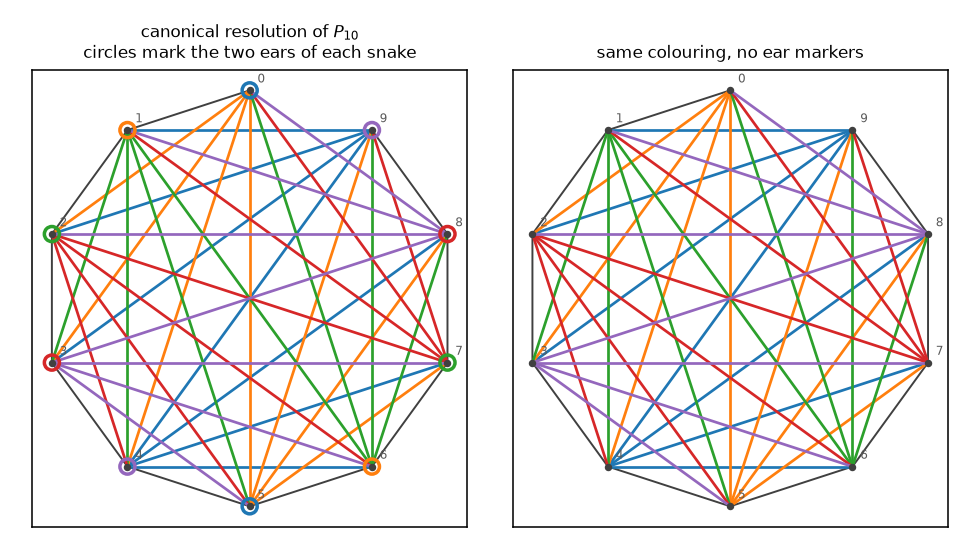
\includegraphics[width=\textwidth]{../figures/fig1_canonical_resolution.png}
\caption{The canonical resolution of $P_{10}$: five snakes, each drawn in its own colour.
Each snake has exactly two ears (circled), and the five ear pairs are the antipodal pairs
$\{0,5\},\dots,\{4,9\}$.}
\label{fig:canonical}
\end{figure}

\begin{figure}[h]
\centering
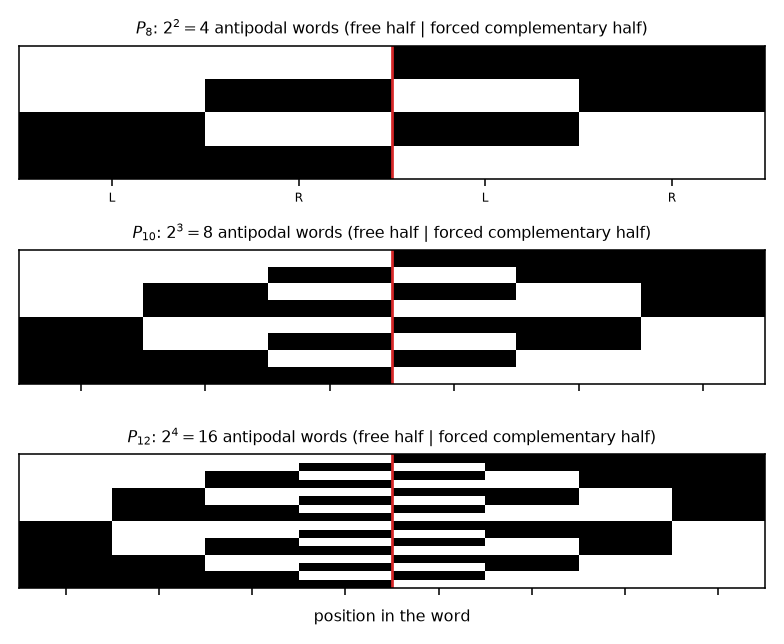
\includegraphics[width=0.75\textwidth]{../figures/fig2_word_enumeration.png}
\caption{All antipodal words of $P_8,P_{10},P_{12}$ as binary matrices ($0=\Li$, $1=\Ri$).
Condition \textup{(CP)} forces the second half to be the letter-wise complement of the
first, which is the reason the count is $2^{m-2}$.}
\label{fig:words}
\end{figure}

\paragraph{Verification of Conjecture C1.}
\Cref{tab:conj} reports, for each $m$, the number of snakes of $P_{2m}$, the number with
non-antipodal ears, and the outcome of testing, for every such non-antipodal snake $S$,
whether $S$ extends to a resolution.  The extension question is the exact-cover problem
``partition $\D_{2m}\setminus S$ into $m-1$ snakes'', i.e.\ an integer program with
$\sum_{T\ni d}y_T=1$ for each remaining diagonal $d$ and $y_T\in\{0,1\}$, solved by HiGHS.
Positive answers are re-validated independently by extracting the witness and re-checking
that it is a partition; no positive answer occurs.  For $m\le5$ the total number of
resolutions is additionally confirmed by exhaustive search over all families of snakes
(agreement with $2^{m-2}$).

\begin{table}[h]
\centering\small
\begin{tabular}{rrrrrl}
\toprule
$m$ & $n$ & \#snakes & \#non-antipodal snakes & resolutions & brute force agrees\\
\midrule
3 & 6  & 12    & 6    & 2  & yes\\
4 & 8  & 64    & 40   & 4  & yes\\
5 & 10 & 320   & 220  & 8  & yes\\
6 & 12 & 1536  & 1116 & 16 & --\\
7 & 14 & 7168  & 5404 & 32 & --\\
\bottomrule
\end{tabular}
\caption{Verification of Conjecture~C1: no snake with non-antipodal ears extends to a
resolution, for every $m\le7$.  The column ``resolutions'' is $2^{m-2}$ by
\cref{cor:count}(ii).}
\label{tab:conj}
\end{table}

\paragraph{Figures.}  \cref{fig:canonical} shows the canonical resolution of $P_{10}$;
\cref{fig:words} shows the anti-palindromic words; further figures (produced by
\texttt{experiments/make\_figures.py}) plot the number of resolutions against $2^{m-2}$,
the exact $k$-packing counts, and the $p$-angulation bound-versus-optimum gap of
\cref{prop:p-angulations}.

\section{Complexity}

\begin{itemize}
\item \emph{Enumeration.}  The recursive enumerator uses $O(1)$ amortised work per
dissection and $O(n)$ memory per stack level; it produces all $C_{n-2}$ triangulations of
$P_n$ in $O(n\,C_{n-2})$ time, which is optimal up to the output size.  In practice it
enumerates $P_{14}$ ($208\,012$ triangulations) and $P_{16}$ ($2\,674\,440$) in seconds.
\item \emph{Packing by integer programming.}  The packing problem has $\binom{n-2}{n-3}$
variables and $n(n-3)/2$ constraints, so its LP relaxation has size $\binom{n-2}{n-3} =
\Theta(4^n/n^{3/2})$.  It is solved exactly for $n\le13$ within seconds.
\item \emph{Certificates.}  Optimality of a packing of size $k$ in $P_n$ is certified by a
family of size $k$ together with the dual solution $x_d=\tfrac12$ on short diagonals and
$0$ elsewhere, of value $n/2$; since every triangulation meets the short diagonals in at
least two members this is a valid LP-dual certificate of the bound
$\lfloor n/2\rfloor$.  (\cref{thm:packing-number} shows that the bound is tight, so no
stronger dual solution exists.)
\item \emph{Counting $k$-packings.}  Backtracking on bit masks over $\binom{n}{2}-n$
diagonals is exponential in the worst case; it is exact up to $n=10$ (the $k=5$ count for
$n=10$ takes about 90 seconds) and is superseded by the classification for $k=n/2$.
\item \emph{Completeness check.}  One integer program per non-antipodal snake; the number of
such snakes is $\Theta(n\,2^{n-5})$, so the check for $m=7$ ($5404$ programs) takes about
five minutes and grows by roughly a factor $4$ with $n$.
\end{itemize}

\section{Discussion}

Three features of the problem are worth emphasising.

\emph{Counting is not enough.}  The diagonal count gives $k\le n/2$ for $P_{2m}$ and the
construction attains it, but for the $p$-angulation variant the same argument leaves a gap
(\cref{prop:p-angulations}).  The ear argument, not the counting argument, is what makes
Theorem 1 sharp, and it is also what forces the rigidity of Proposition~\ref{prop:structure}.

\emph{The classification is one line long once the right encoding is found.}  Encoding a
snake as a word (\cref{lem:strip}) and observing that the level of the $i$-th strip diagonal
does not depend on the word reduces the covering problem to a condition on two blocks of
consecutive residues, which is equivalent to a single anti-palindromicity requirement.  The
resulting count $2^{m-2}$ is far smaller than the number of snakes, and the structure of the
answer (\cref{fig:words}) is completely transparent.

\emph{Where the proof stops.}  The natural next step, Conjecture C1, is the statement that
the classification is exhaustive.  The gap is localised (see \cref{sec:limits}): the
covering argument needs the starts at a fixed level to form two blocks of consecutive
residues, which is automatic only when all snakes share a word.  Our partial analysis shows
the sharing is forced at the first and the last move and (with a parity caveat) at the
second moves; completing the induction is the concrete open problem.

\section{Future work}

\begin{enumerate}
\item Prove or refute Conjecture C1.  A positive answer gives the exact count $2^{m-2}$ of
resolutions of $P_{2m}$; a negative answer would exhibit a resolution with a non-antipodal
ear configuration, which our searches for $m\le7$ did not find.
\item Determine the maximum number of pairwise edge-disjoint $p$-angulations of $P_n$ for
$p\ge4$ and $n$ large; for quadrilaterals the exact values for $n\le10$ are $1,3,4,5$ for
$n=4,6,8,10$, and the general answer is unknown to us.
\item Study the non-convex case: for a simple $n$-gon the number of triangulations varies
wildly (from $1$ to $C_{n-2}$), and the analogue of Theorem 1 should involve the number of
\emph{dissectible} diagonals rather than $n$.
\item Relate the resolution structure to cluster algebras: triangulations of a convex
$2m$-gon with the same word form an "interval" in a Tamari- or Cambrian-type lattice, and
the $m$ snakes of a resolution might correspond to a maximal antichain or to an
almost-complete positive sequence in a rank-$2$ cluster algebra.
\end{enumerate}

\section{Conclusion}

We determined the maximum number of pairwise edge-disjoint triangulations of a convex
polygon to be $\lfloor n/2\rfloor$, proved that for even $n$ every extremal family is a
partition of all diagonals into snakes with pairwise disjoint ear pairs, and classified the
resolutions whose snakes follow a common word --- these are automatically antipodal, and
there are exactly $2^{m-2}$ of them for $P_{2m}$, in bijection with binary words of length
$m-2$.  The classification rests on a
new and useful encoding of snakes as lattice paths, which also yields the count
$n\,2^{n-5}$ of snakes and makes the level structure of a snake visible.  Exhaustive
computation verifies that every resolution of $P_{2m}$ follows a common word for $m\le7$
(polygons up to $P_{14}$); we conjecture the remaining case and locate precisely the step of
the proof that fails.

\begin{thebibliography}{9}
\bibitem{huangfu2018}
Q.~Huangfu and J.~A.~J.~Hall.
\newblock Parallelizing the dual revised simplex method.
\newblock \emph{Mathematical Programming Computation}, 10(1):119--142, 2018.

\bibitem{virtanen2020}
P.~Virtanen, R.~Gommers, T.~E.~Oliphant, et~al.
\newblock SciPy 1.0: fundamental algorithms for scientific computing in Python.
\newblock \emph{Nature Methods}, 17(3):261--272, 2020.

\bibitem{oeisA000108}
OEIS~A000108, Catalan numbers.
\newblock \url{https://oeis.org/A000108}
\end{thebibliography}

\appendix

\section{Explicit resolutions of small polygons}\label{app:examples}

For $n=6$ the two resolutions (words $\Li\Ri$ and $\Ri\Li$) are
\[
  \{\{(1,3),(1,4)\},\;\{(0,2),(2,4)\},\;\{(0,3),(3,5)\}\}
  \quad\text{and}\quad
  \{\{(1,4),(2,4)\},\;\{(0,2),(0,3)\},\;\{(1,3),(1,4)\}\}.
\]
For $n=8$ the four words are $\Li\Li\Ri\Ri,\ \Li\Ri\Li\Ri,\ \Ri\Li\Ri\Li,\
\Ri\Ri\Li\Li$, i.e.\ the first $m-2=2$ letters are free.  The library prints any of them:

\begin{verbatim}
>>> import edd
>>> res = edd.antipodal_resolutions(8)[1]        # word "LRLR"
>>> res.word, len(res)
('LRLR', 4)
>>> sorted(sorted(T) for T in res)              # doctest: +NORMALIZE_WHITESPACE
[[(0, 2), (2, 7), (3, 6), (3, 7), (4, 6)], [(0, 3), (0, 4), (1, 3), (4, 7), (5, 7)],
 [(0, 5), (0, 6), (1, 4), (1, 5), (2, 4)], [(1, 6), (1, 7), (2, 5), (2, 6), (3, 5)]]
>>> edd.count_resolutions(8), edd.brute_force_count_resolutions(8)
(4, 4)
\end{verbatim}

\section{Reproduction}

\begin{verbatim}
pip install -e .
python -m pytest tests -q          # 188 tests
python experiments/run_all.py      # regenerates results/ and figures/
\end{verbatim}
The only numerical ingredient is HiGHS (through \textsc{scipy}); every other computation is
exact integer arithmetic.  The completeness check for $m=8$ is available with
\texttt{python experiments/run\_all.py --full} but was not run for the tables in this
repository, which stop at $m=7$.

\end{document}